%\documentclass[handout]{beamer}
\documentclass[lecture]{beamer}

%\usepackage[latin1]{inputenc}
\usepackage{pifont,amsmath,amssymb,amsfonts,euscript,mathrsfs,wasysym,textcomp}
\usepackage{psfrag}
\usepackage{multimedia}
\usepackage{fancybox}
\usepackage{soul}
\usetheme{Boadilla}
\usepackage{xcolor}

\usepackage{array}
\usepackage{calc}

\usepackage{pgf}
\usepackage{tikz}
\usetikzlibrary{decorations.markings}

\usepackage[utf8]{inputenc}
\usetikzlibrary{arrows,automata}
\usetikzlibrary{positioning}
\usetikzlibrary{calc}
\usepackage{amsmath}

\newcommand {\cmatr}[2]{\left\{\begin{array}{#1}#2\end{array}\right.}

\makeatletter
\newcommand{\pushright}[1]{\ifmeasuring@#1\else\omit\hfill$\displaystyle#1$\fi\ignorespaces}
\newcommand{\pushleft}[1]{\ifmeasuring@#1\else\omit$\displaystyle#1$\hfill\fi\ignorespaces}
\makeatother

\DeclareMathOperator*{\argmax}{arg\,max}
\DeclareMathOperator*{\argmin}{arg\,min}



\newcommand{\highlightred}[1]{%
  \colorbox{red!50}{$\displaystyle#1$}}
  \newcommand{\highlightgreen}[1]{%
  \colorbox{green!50}{$\displaystyle#1$}}
\usepackage{pgfpages}
%\pgfpagesuselayout{4 on 1}[a4paper,landscape,border shrink=5mm]
%\pgfpagesuselayout{2 on 1}[letterpaper,border shrink=5mm]
\usepackage{mathtools}

\setbeamertemplate{blocks}[rounded][shadow=false]

\newtheorem{Proposition}{Proposition}

\usepackage{tikz}
\usetikzlibrary{arrows,shapes}
\tikzstyle{na} = [baseline=-.5ex]
\tikzstyle{every picture}+=[remember picture]
\usetikzlibrary{positioning,intersections}

\makeatletter
\def\hlinewd#1{%
\noalign{\ifnum0=`}\fi\hrule \@height #1 %
\futurelet\reserved@a\@xhline}
\makeatother



\newsavebox{\fmbox}
\newenvironment{fmpage}[1]
  {\begin{lrbox}{\fmbox}\begin{minipage}{#1}}
  {\end{minipage}\end{lrbox}\fbox{\usebox{\fmbox}}}

\newcommand\BackgroundPicture[1]{%
   \setbeamertemplate{background}{%
   \parbox[c][\paperheight]{\paperwidth}{%
       \vfill \hfill
        \includegraphics[width=1\paperwidth,height=1\paperheight]{#1}
        \hfill \vfill
}}}

\definecolor{myGreen}{rgb}{0.,0.4,0.}
\definecolor{myGreen2}{rgb}{0.,0.8,0.}
\definecolor{myGreen3}{rgb}{0.,0.6,0.}
\definecolor{myLightGreen}{rgb}{0.9,1,0.9}
\definecolor{myBlue}{rgb}{0.,0.,0.4}
\definecolor{myBlue2}{rgb}{0,0.1,0.6}
\definecolor{myOrange}{rgb}{1.,0.5,0.}
\definecolor{myBrown}{rgb}{.65,.16,.15}
\definecolor{myCyan}{rgb}{.65,.16,.15}
\definecolor{myPurple}{rgb}{1,0,1}
\definecolor{myRed}{rgb}{0.8,0,0}
\definecolor{myRed2}{rgb}{0.65,0,0}
\definecolor{deepBlue}{rgb}{0.0,0,1}
\definecolor{myMagenta}{rgb}{0.7,0,0.8}


\definecolor{myLightBlue}{rgb}{0.9,0.9,1}
\definecolor{myLightRed}{rgb}{1,0.9,0.9}


\newcommand{\FSII}{1}
\newcommand{\FSIII}{0.8}




\newcommand {\condmatr}[2]{\left\{\begin{array}{#1}#2\end{array}\right.}
\newcommand{\defi}{\stackrel{\footnotesize\Delta}{=}}
\newcommand{\expon}[1]{\ensuremath{\textnormal{e}^{#1}}}
\newcommand{\RR}{\textnormal{\textsf{I}\!\textsf{R}}}
\newcommand{\ini}[1]{\ensuremath{#1_{k}}}
\newcommand{\fin}[1]{\ensuremath{#1_\textnormal{f}}}
\newcommand{\der}[1]{\textnormal{d}{#1}}
\newcommand{\derk}[2]{\textnormal{d}^{#1}#2}
\newcommand{\ddt}[1]{\frac{\der{#1}}{\der{t}}} 
\newcommand{\dkdtk}[2]{\frac{\derk{#1}{#2}}{\der{t}^{#1}}} 
\newcommand{\dd}[2]{\frac{\der{#1}}{\der{#2}}} 
\newcommand{\NN}{\ensuremath{\textnormal{\textsf{I}\!\textsf{N}}}}
\newcommand {\matr}[2]{\left[\begin{array}{#1}#2\end{array}\right]}
\newcommand {\omatr}[2]{\begin{array}{#1}#2\end{array}}
%\newcommand{\Rn}[1]{\ensuremath{\RR^{#1}}}
%\newcommand{\En}[1]{\ensuremath{E_{#1}}}
\newcommand{\En}[1]{\ensuremath{\RR^{#1}}}
\newcommand{\R}[1]{\ensuremath{\RR^{#1}}}
\newcommand{\lagr}{\ensuremath{\mathcal{L}}}
\newcommand{\hamil}{\ensuremath{\mathcal{H}}}
\newcommand{\hamax}{\ensuremath{\mathcal{M}}}
\newcommand{\ndxset}{\ensuremath{\EuScript{K}}}
\newcommand{\id}[1]{\ensuremath{I_{#1}}}
%\newcommand{\matr}[1]{\ensuremath{\textnormal{\sf #1}}}
\newcommand{\vect}[1]{\ensuremath{\boldsymbol{\mathrm{#1}}}}
\newcommand{\const}[1]{\ensuremath{\overline{#1}}}
\newcommand{\fixed}[1]{\ensuremath{\underline{#1}}}
\newcommand{\transp}[1]{\ensuremath{{#1}^\textnormal{\textsf{T}}}}
\newcommand{\invtr}[1]{\ensuremath{{#1}^{-\textnormal{\textsf{T}}}}}
\newcommand{\inv}[1]{\ensuremath{#1^{-1}}}
\newcommand{\inter}[1]{\ensuremath{\textnormal{int}\left({#1}\right)}}
\newcommand{\closur}[1]{\ensuremath{\textnormal{cl}\left({#1}\right)}}
\newcommand{\rank}[1]{\ensuremath{\oprank\left({#1}\right)}}
\newcommand{\diag}[1]{\ensuremath{\opdiag\left({#1}\right)}}
\renewcommand{\ker}[1]{\ensuremath{\opker\left({#1}\right)}}
\renewcommand{\det}[1]{\ensuremath{\opdet\left({#1}\right)}}
\newcommand{\opt}[1]{{#1}^\star}
\newcommand{\nom}[1]{{#1}^\star}
\newcommand{\pert}[1]{{#1}^\dagger}
\newcommand{\activ}[2]{\ensuremath{\EuScript{A}_{#1}\left(#2\right)}}
\newcommand{\ball}[2]{\ensuremath{\EuScript{B}_{#1}\left(#2\right)}}
\newcommand{\iball}[3]{\ensuremath{\EuScript{B}_{#1}^{#2}\left(#3\right)}}
\newcommand{\cball}[2]{\ensuremath{\bar{\EuScript{B}}_{#1}\left(#2\right)}}
\newcommand{\dball}[2]{\ensuremath{\dot{\EuScript{B}}_{#1}\left(#2\right)}}
\newcommand{\boun}[1]{\ensuremath{\partial #1}}
\newcommand{\C}[1]{\ensuremath{\mathcal{C}^{#1}}}
\newcommand{\PWC}[1]{\ensuremath{\hat{\mathcal{C}}^{#1}}}
\newcommand{\proj}[2]{\ensuremath{\mathcal{P}_{#1}#2}}
\newcommand{\F}{\ensuremath{\EuScript{F}}}
\newcommand{\J}{\ensuremath{\EuScript{J}}}
\newcommand{\D}{\ensuremath{\EuScript{D}}}
\newcommand{\X}{\ensuremath{\EuScript{X}}}
\newcommand{\K}{\ensuremath{\EuScript{K}}}
\newcommand{\U}{\ensuremath{\EuScript{U}}}
\newcommand{\V}{\ensuremath{\EuScript{V}}}
\renewcommand{\P}{\ensuremath{\EuScript{P}}}
\newcommand{\ext}[1]{\ensuremath{\tilde{#1}}}
\newcommand{\tang}{\ensuremath{\mathscr{T}}}
\newcommand{\impdir}[1]{\ensuremath{\mathscr{D}}(#1)}
\newcommand{\feasdir}[2]{\ensuremath{F}_{#1}\left(#2\right)}
%\newcommand{\activ}[1]{\ensuremath{\EuScript{A}(#1)}}
\newcommand{\dc}{c}
\newcommand{\RK}{\ensuremath{\textnormal{RK}}}

\newcommand{\intP}{\vect{P}}
\newcommand{\intXk}{X}
\newcommand{\intX}{\vect{\intXk}}
\newcommand{\x}{{\bf x}}
\newcommand{\y}{{\bf y}}
\newcommand{\p}{{\bf p}}
\newcommand{\q}{{\bf q}}
\newcommand{\term}{\phi}
\newcommand{\integ}{\psi}
\newcommand{\ODEi}{f}
\newcommand{\ODE}{\vect{\ODEi}}
\newcommand{\ODECVXi}[1]{u_{f_{#1}}}
\newcommand{\ODECVX}{\vect{\ODECVXi{}}}
\newcommand{\ODECCVi}[1]{o_{f_{#1}}}
\newcommand{\ODECCV}{\vect{\ODECCVi{}}}
\newcommand{\ICi}[1]{h_{#1}}
\newcommand{\IC}{\vect{\ICi{}}}
\newcommand{\ICCVXi}[1]{u_{h_{#1}}}
\newcommand{\ICCVX}{\vect{\ICCVXi{}}}
\newcommand{\ICCCVi}[1]{o_{h_{#1}}}
\newcommand{\ICCCV}{\vect{\ICCCVi{}}}

\newcommand{\lb}[1]{#1^{\rm L}}
\newcommand{\ub}[1]{#1^{\rm U}}
\newcommand{\cv}[1]{\vect{u}_{#1}}
\newcommand{\cc}[1]{\vect{o}_{#1}}
\newcommand{\dcv}[1]{\dot{\vect{u}}_{#1}}
\newcommand{\dcc}[1]{\dot{\vect{o}}_{#1}}
\newcommand{\cvi}[1]{u_{#1}}
\newcommand{\cci}[1]{o_{#1}}
\newcommand{\trace}[1]{\text{Tr}\left(#1\right)}

\DeclareMathOperator{\esssup}{ess\,sup}
\DeclareMathOperator{\essinf}{ess\,inf}
\DeclareMathOperator{\sign}{sign}
\DeclareMathOperator{\oprank}{rank}
\DeclareMathOperator{\opker}{ker}
\DeclareMathOperator{\opdet}{det}
\DeclareMathOperator{\opdiag}{diag}
\DeclareMathOperator{\midf}{mid}
\DeclareMathOperator{\opcard}{card}

\definecolor{myGreen}{rgb}{0.,0.4,0.}
\definecolor{myGreen2}{rgb}{0.,0.8,0.}
\definecolor{myGreen3}{rgb}{0.,0.6,0.}
\definecolor{myBlue}{rgb}{0.,0.,0.4}
\definecolor{myBlue2}{rgb}{0,0.1,0.8}
\definecolor{myOrange}{rgb}{1.,0.5,0.}
\definecolor{myOrange2}{rgb}{0.8.,0.5,0.}
\definecolor{myBrown}{rgb}{.65,.16,.15}
\definecolor{myCyan}{rgb}{.65,.16,.15}
\definecolor{myPurple}{rgb}{1,0,1}
\definecolor{myRed}{rgb}{0.8,0,0}
\definecolor{myRed3}{rgb}{1,0.7,0.7}

\usetikzlibrary{arrows,positioning,calc}

\usepackage[ruled,vlined]{algorithm2e}
\renewcommand{\thealgocf}{}
\newtheorem {Algorithm}{Algorithm}
\SetAlCapFnt{\scriptsize}
\usepackage{caption}

\usepackage{tikz}
\usetikzlibrary{positioning,arrows}
\tikzset{
    state/.style={
           rectangle,
           rounded corners,
           draw=black, very thick,
           minimum height=2em,
           inner sep=2pt,
           text centered,
           },
}

%\AtBeginSection[]
%{
%{\usebackgroundtemplate{
% \parbox[c][\paperheight][b]{\paperwidth}{
%    \flushright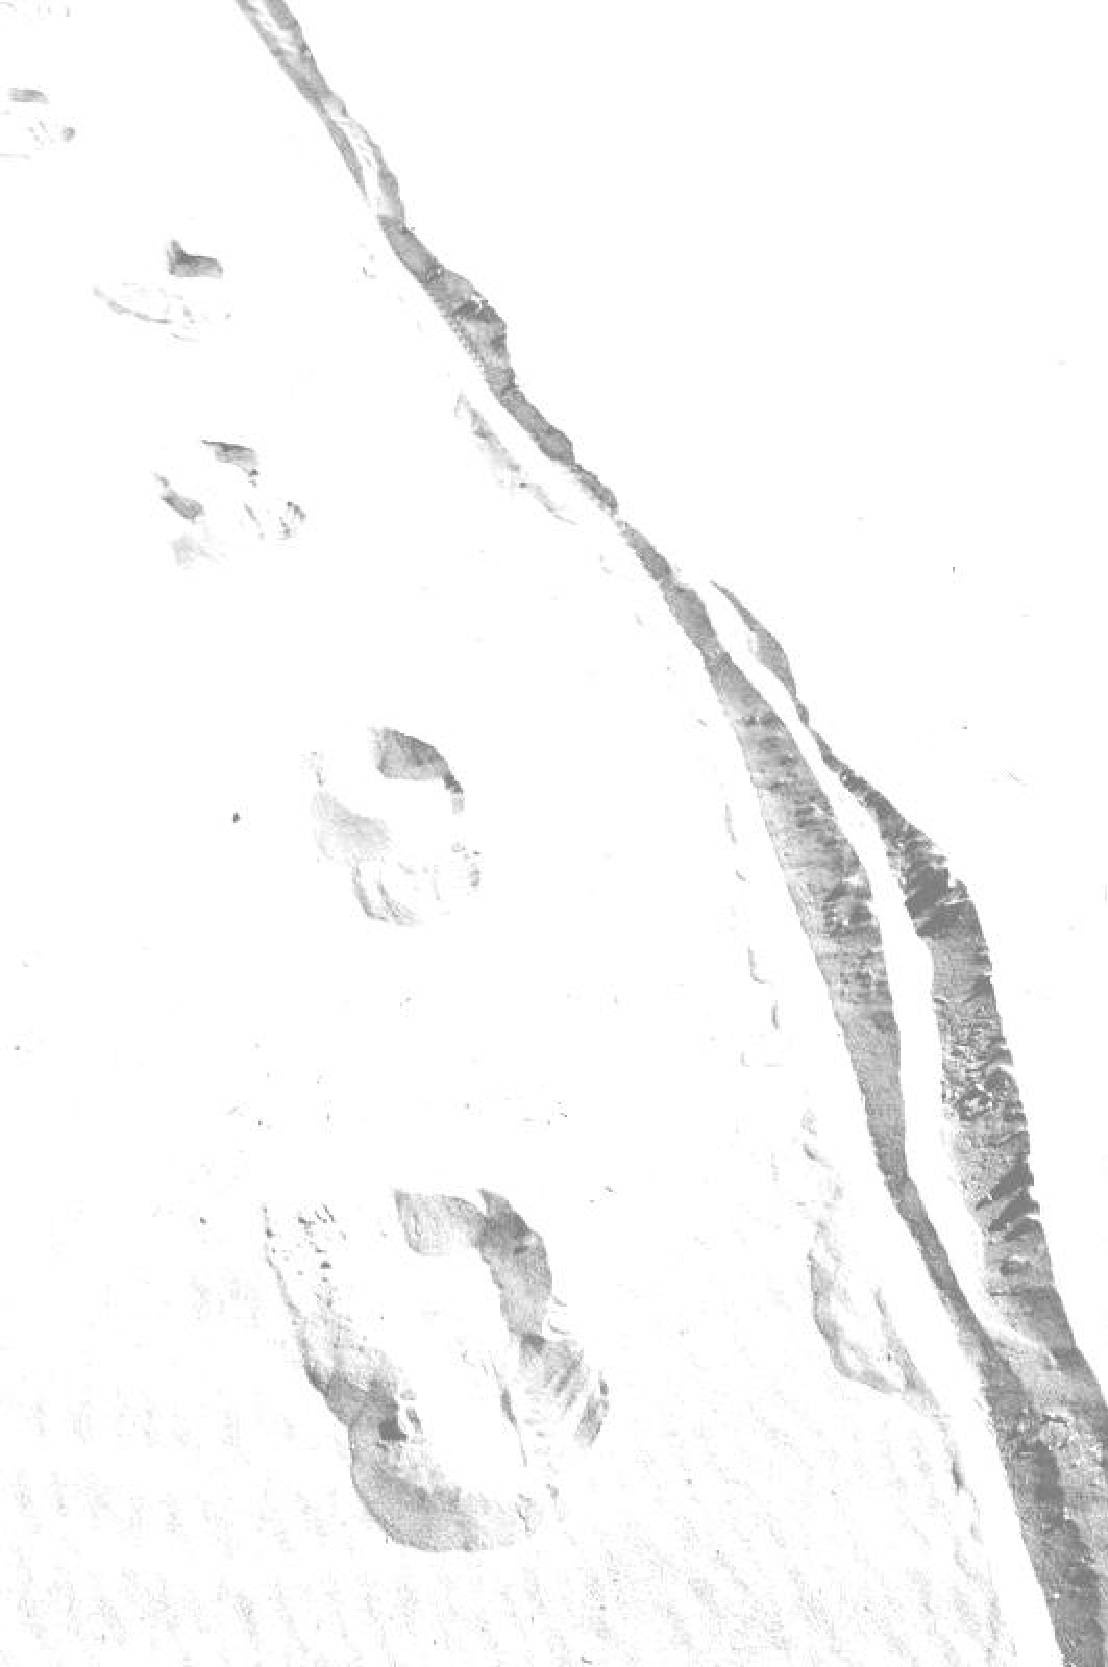
\includegraphics[width=0.55\paperwidth, height = \paperheight]{Figures/Track.pdf}}}
%  \begin{frame}{\normalsize Outline}
%  \tableofcontents[currentsection]
%  \end{frame}}
%}



\title[RloverRL]{Closing Sim2Real Gap via Bi-level Reinforcement Learning}
\author[Akhil S Anand]{\large Akhil S Anand}
\institute[NTNU]{Department of Engineering Cybernetics \\ Faculty of Information Technology \\  NTNU}
\date[18 September 2025]
% {$1^\mathrm{st}$ AID Scientific Workshop, Trondheim}

%%%%%%%%%%%%%%%%%%%%%%%%%%%%%%%%%%%%%%%%%%%%%%%%%%%%%%%%%%%%%%%%%%%%%%%%

\begin{document}


%


%{\usebackgroundtemplate{
% \parbox[c][\paperheight][b]{\paperwidth}{
%    \flushright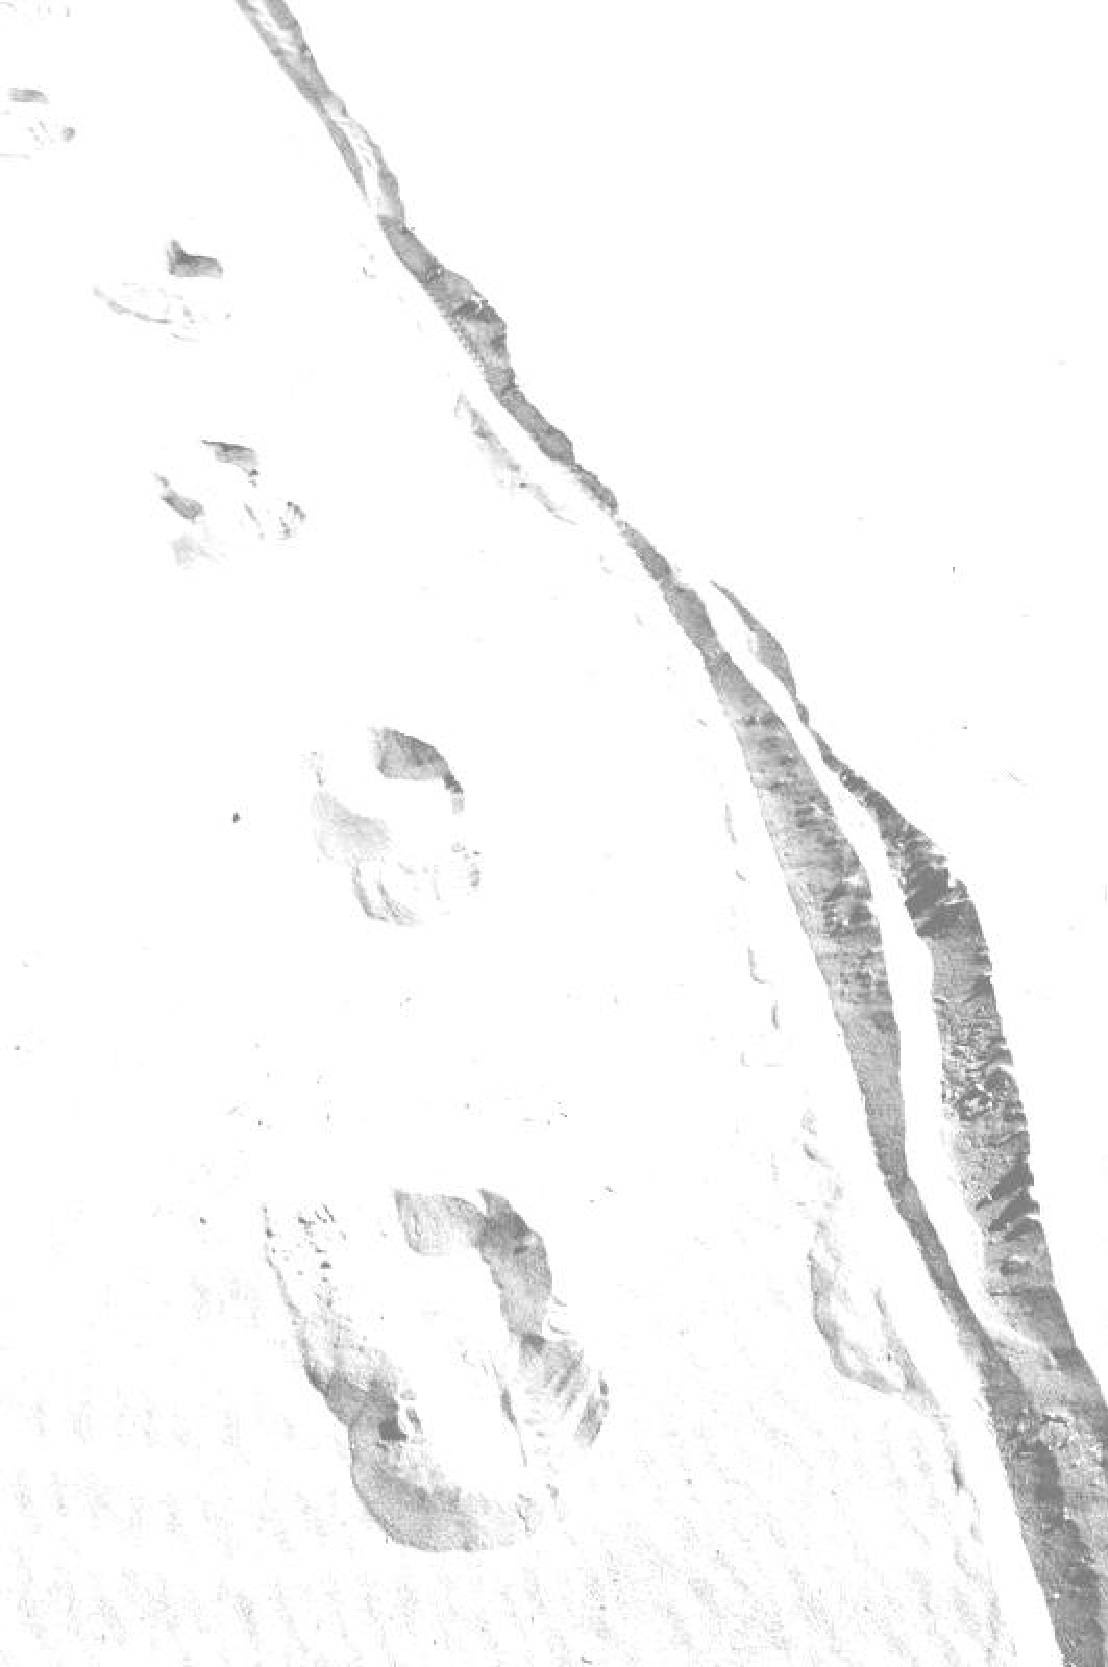
\includegraphics[width=0.55\paperwidth, height = 1\paperheight]{Figures/Track.pdf}}}
%\begin{frame}
%\titlepage
%\end{frame}}







       
% RL-over-RL Motivation and Bi-Level Formulation

\section{RL-over-RL Motivation and Bi-Level Formulation}

\begin{frame}{\normalsize Closing Sim2Real gap via Bi-level RL}
\footnotesize
\only<1>{
  \begin{overlayarea}{\textwidth}{7cm}
\begin{itemize}
\item Sim2Real Gap:
\begin{itemize}
  \item Improving simulator accuracy and robustness.
  \item Accuracy and robustness does not guarantee optimal real-world performance.
  \item Optimize simulator parameters \(\theta\) to maximize real-world return.
\end{itemize}
\end{itemize}
\end{overlayarea}
}
\only<2->{
\centering
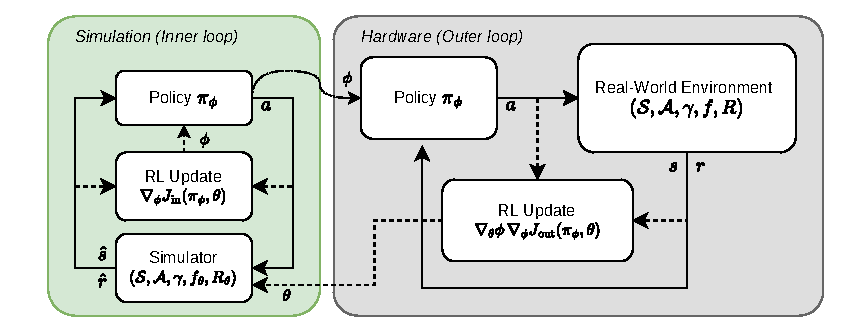
\includegraphics[width=\textwidth]{Figures/rl_over_rl_overview.pdf}

This leads to a {bi-level optimization problem}:
\[
\max_{\theta} \; J(\pi_{\phi(\theta)}, \; \text{real world}) 
\quad \text{s.t.}\quad 
\phi(\theta) = \arg\max_{\phi} \; \hat J(\pi_\phi, f_\theta,R_\theta).
\]
}

\only<3-4>{
\begin{itemize}
\item \textbf{Inner level:} In-sim RL (SPG) finds \(\pi_\phi\) optimal for simulator.
\item \textbf{Outer level:} Updates simulator parameters \(\theta\) to improve real-world performance.
\end{itemize}
}

\only<4->{
\[
\nabla_\theta J_{\text{real}}\!\big(\pi_{\phi(\theta)}\big)
\;=\;
\underbrace{\nabla_\theta \phi(\theta)}_{\text{policy sensitivity}}
\;
\underbrace{\mathbb{E}_{s\sim \rho^{\pi_\phi},\,a\sim\pi_\phi(\cdot|s)}
\!\big[\,\nabla_\phi \log \pi_\phi(a|s)\; Q^{\pi_\phi}(s,a)\big]}_{\text{policy gradient (real world)}}.
\]}

\only<5->{
\(\nabla_\theta \phi\): To compute outer gradients, we need how the inner policy \(\pi_\phi\) changes when simulator parameters \(\theta\) are perturbed.}
\end{frame}



\begin{frame}{\normalsize Sensitivity of In-Sim RL}
\footnotesize

\begin{itemize}
\item Inner SPG defines an implicit condition:
\(\hat\phi(\phi,\theta) = \mathbb{E}_{\hat\rho^{\pi_\phi}_\theta}\!\big[\nabla_\phi \log \pi_\phi \; \hat Q^{\pi_\phi}_\theta\big] = 0.\)
\item \(\nabla_\theta \phi\) using the {Implicit Function Theorem} applied to this condition.
\item Conceptually, this requires:
  \begin{enumerate}\footnotesize
  \item Estimating the sensitivity of the markov chain of the simulator under a policy w.r.t. \(\theta\).
  \item Estimating the sensit of in-sim critic w.r.t simulator parameters \(\theta\).
  \item Combining these to obtain the sensitivity of in-sim policy: \(\nabla_\theta \phi\)
  \end{enumerate}
\item In practice, these quantities can be estimated using in-sim rollouts (no need for real-world exploration).
\item Combine real-world PG with the in-sim sensitivities to update $\theta$ for better real return.
\end{itemize}


\end{frame}



\begin{frame}{\normalsize Differentiating the Markov Chain}
\footnotesize
Sensitivity of a Markov chain expectation: Differentiate an expectation at a fixed step \(k\) under the in-sim Markov chain.\\[0.1cm]
\begin{align*}
\partial \, \mathbb E_{s\sim \hat\rho_{\theta,k}^{\pi_{\phi}}} \bigl[\eta(s_k,a_k)\bigr] 
= \mathbb{E}_{\substack{s_0\sim\rho^0,\,a_i\sim\pi_\phi,\\s_{i+1}\sim f^{\pi_\phi}_{\theta}}}
   \Bigl[\,
     \eta(s_k,a_k)\,\Bigl(
        \partial\log\pi_\phi(a_k\!\mid\!s_k)
      + \sum_{i=0}^{k-1}\partial\log f^{\pi_\phi}_{\theta}(s_{i+1}\!\mid\!s_i,a_i)
     \Bigr)
   \Bigr]\,.
\end{align*}

\centering 
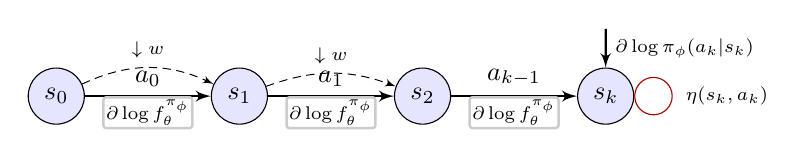
\begin{tikzpicture}[>=latex',node distance=1.05cm,scale=0.95, every node/.style={scale=0.95}]
\tikzstyle{st}=[circle, draw=black, fill=myLightBlue, minimum size=0.75cm, inner sep=0pt]
\tikzstyle{edge}=[->, line width=0.9pt]
\tikzstyle{edgeThin}=[->, line width=0.35pt, densely dashed]
\tikzstyle{lbl}=[font=\scriptsize, inner sep=1pt, fill=white, draw=black!20, rounded corners=1pt]
% chain backbone
\node[st] (s0) {$s_0$};
\node[st, right=1.6cm of s0] (s1) {$s_1$};
\node[st, right=1.6cm of s1] (s2) {$s_2$};
\node[st, right=1.6cm of s2] (sk) {$s_k$};
% main (upweighted) path
\draw[edge] (s0) -- node[above] {$a_0$} node[lbl, below] {$\partial\log f_\theta^{\pi_\phi}$} (s1);
\draw[edge] (s1) -- node[above] {$a_1$} node[lbl, below] {$\partial\log f_\theta^{\pi_\phi}$} (s2);
\draw[edge] (s2) -- node[above] {$a_{k-1}$} node[lbl, below] {$\partial\log f_\theta^{\pi_\phi}$} (sk);
% alternative (downweighted) branches
\path (s0) edge[edgeThin, bend left=25] node[above] {\scriptsize $\downarrow w$} (s1);
\path (s1) edge[edgeThin, bend left=20] node[above] {\scriptsize $\downarrow w$} (s2);
% action score at step k
\draw[->, thick] ($(sk)+(0,0.9)$) -- (sk) node[midway, right] {\scriptsize $\partial\log\pi_\phi(a_k|s_k)$};
% eta marker
\node[draw=myRed2, circle, inner sep=1pt, minimum size=0.5cm, right=0.0cm of sk] (eta) {};
\node[font=\scriptsize, right=0.05cm of eta] {$\eta(s_k,a_k)$};
\end{tikzpicture}
\vspace{0.1cm}

\begin{itemize}
  \item The sensitivity estimation amounts to reweighting each trajectory by how its likelihood changes under $\partial$ and adjusting at step $k$ for the chosen action.
\end{itemize}


\end{frame}

\begin{frame}{\normalsize Differentiating the Critic }
\footnotesize
The critic satisfies a fixed point under the bellman operator; change in $\theta$ perturbs \emph{every} backup along the trajectory tree.\\[0.15cm]
\begin{align*}
\partial Q^{\pi}(s,a)&= \partial R(s,a)+\gamma\mathbb E_{s_+ \sim f}\left[\partial V^{\pi}(s_+) + V^{\pi}(s_+)\partial\log f(s_+|s,a)\right],\\
\partial V^{\pi}(s)&=\mathbb E_{a\sim\pi}\left[\partial Q^{\pi}(s,a)+Q^{\pi}(s,a)\partial\log\pi(a|s)\right].
\end{align*}

\begin{columns}[T]
\column{0.5\textwidth}
\begin{itemize}
\item Start at $Q(s_t,a_t)$.
\item A small $\delta\theta$ 
  \begin{enumerate}
    \footnotesize
  \item perturbs $R_\theta(s_t,a_t)$ (local),
  \item re-weights next states via $f_\theta$ (global),
  \item and keeps propagating through $V(s_{t+1})$, $V(s_{t+2})$, \dots
  \end{enumerate}
\end{itemize}

\column{0.5\textwidth}
\centering
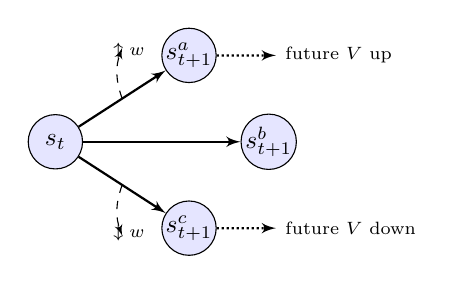
\begin{tikzpicture}[>=latex',node distance=0.8cm,scale=0.92, every node/.style={scale=0.92}]
\tikzstyle{st}=[circle, draw=black, fill=myLightBlue, minimum size=0.75cm, inner sep=0pt]
\tikzstyle{edge}=[->, thick]
\node[st] (s0) {$s_t$};
\node[st, above right=0.6cm and 1.2cm of s0] (s1a) {$s_{t+1}^a$};
\node[st, right=2.0cm of s0] (s1b) {$s_{t+1}^b$};
\node[st, below right=0.6cm and 1.2cm of s0] (s1c) {$s_{t+1}^c$};
\draw[edge] (s0) -- (s1a);
\draw[edge] (s0) -- (s1b);
\draw[edge] (s0) -- (s1c);
% weight changes
\draw[->, dashed] ($(s0)!0.5!(s1a)$) to[bend left=20] +(0,0.7);
\draw[->, dashed] ($(s0)!0.5!(s1c)$) to[bend right=20] +(0,-0.7);
\node at ($(s0)!0.55!(s1a)+(0,0.6)$) {\scriptsize $\uparrow w$};
\node at ($(s0)!0.55!(s1c)+(0,-0.6)$) {\scriptsize $\downarrow w$};
% value arrows
\draw[edge, densely dotted] (s1a) -- +(1.2,0) node[right] {\scriptsize future $V$ up};
\draw[edge, densely dotted] (s1c) -- +(1.2,0) node[right] {\scriptsize future $V$ down};
\end{tikzpicture}

{\scriptsize  $\delta\theta$ changes edge weights (transition probs), so the Bellman backup shifts via both reward and where we go next.}
\end{columns}
\begin{itemize}
\item Immediate effect: rewards $R_\theta(s,a)$ shift with $\theta$.
\item Propagated effect: transition shifts alter \emph{who} we next visit $\Rightarrow$ future values change.
\item The overall sensitivity is a \textit{backward} accumulation along edges of the trajectory tree.
\end{itemize}

\end{frame}

\end{document}

